\section{Langkah-Langkah Percobaan}
\subsection{Crimping}
\begin{enumerate}
    \item Kupas layer terluar kabel UTP sepanjang seruas jari (~4cm).
    \item Pastikan semua kabel tidak terluka.
    \item Meluruskan 8 kabel dan mengurutkan 8 kabel tersebut dalam konfigurasi T-568B.
    \item 8 kabel yang sudah diurutkan dapat dimasukan kedalam konektor RJ45.
    \item Menjepit kabel tersebut pada RJ45 dengan menggunakan Tang Crimping RJ45.
    \item Test hasil crimpingan dengan menggunakan LAN Tester. Jika lampu LED dari 1 sampai dengan 8 menyala secara bergantian.
\end{enumerate}

\subsection{Static Routing}
\begin{enumerate}
    \item Hubungkan kabel LAN dengan Laptop dan buka WinBox pada Laptop.
    \item Pilih menu Neighbours pada WinBox untuk menampilkan Router yang sedang terhubung dan pilih MAC address router serta kilk tombol connect.
    \item Pada menu utama, buka menu System serta pilih restart configuration. Centang No Default Configuration dan kilk Reset Configuration.
    \item Tunggu router restart dan kembali hubungkan router dengan WinBox.
    \item Hubungkan Router 1 dengan Router 2 via kabel LAN pada port ether7 serta ether6 ke laptop.
    \item Pada WinBox, buka menu IP dan pilih Address list. Tekan tombol (+) dan masukan Address dari router yang sedang dikonfigurasi (10.10.10.1/30) pada network antar router (10.10.10.0) dan pilih interface yaitu ether7 (LAN antar router).
    \item Tambah Address lagi untuk laptop pada network yang berbeda serta pilih interface yang digunakan.
        \begin{figure}[H]
            \centering
            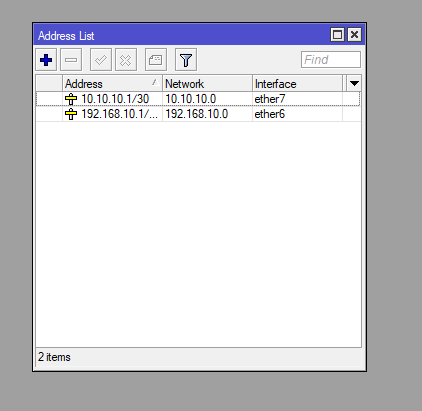
\includegraphics[width=0.5\linewidth]{P1/img/address list static.png}
            \caption{Address List Router 1}
            \label{fig:enter-label}
        \end{figure}
    \item Lakukan hal yang sama pada router ke 2.
        \begin{figure}[H]
            \centering
            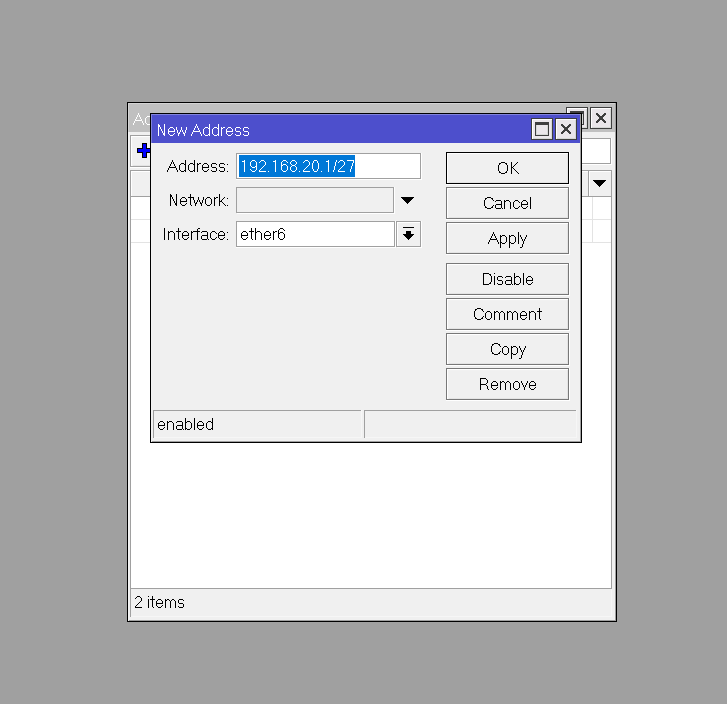
\includegraphics[width=0.35\linewidth]{P1/img/Address Laptop Router 2.png}
            \caption{Address Laptop Router 2}
            \label{fig:enter-label}
        \end{figure}
        \begin{figure}[H]
            \centering
            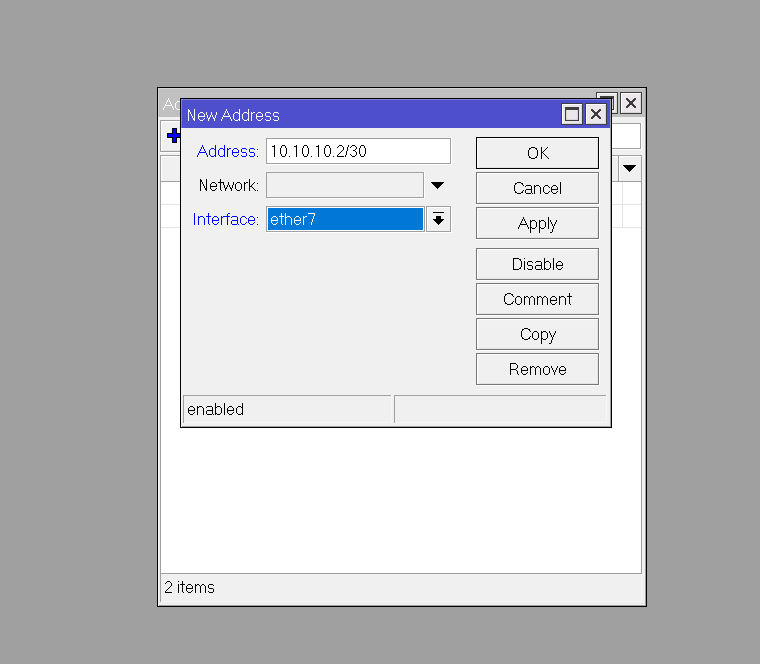
\includegraphics[width=0.35\linewidth]{P1/img/Address Router Router 2.png}
            \caption{Address Router 2}
            \label{fig:enter-label}
        \end{figure}
    \item Pada WinBox, buka menu IP dan pilih Routes.
    \item Klik tombol (+) untuk menambahkan Routing. Dst Address diisi dengan Network Address yang dituju (Router 1 -> 192.168.20.0/27 / Router 2 -> 192.168.10.0/27). Gateway diisi dengan gateway destination (Router 1 -> 10.10.10.2 / Router 2 -> 10.10.10.1).
        \begin{figure}[H]
            \centering
            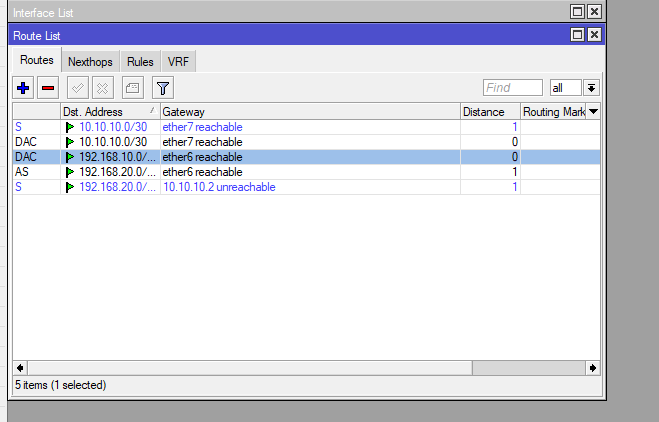
\includegraphics[width=0.5\linewidth]{P1/img/route list statis.png}
            \caption{Route List 1}
            \label{fig:enter-label}
        \end{figure}
        \begin{figure}[H]
            \centering
            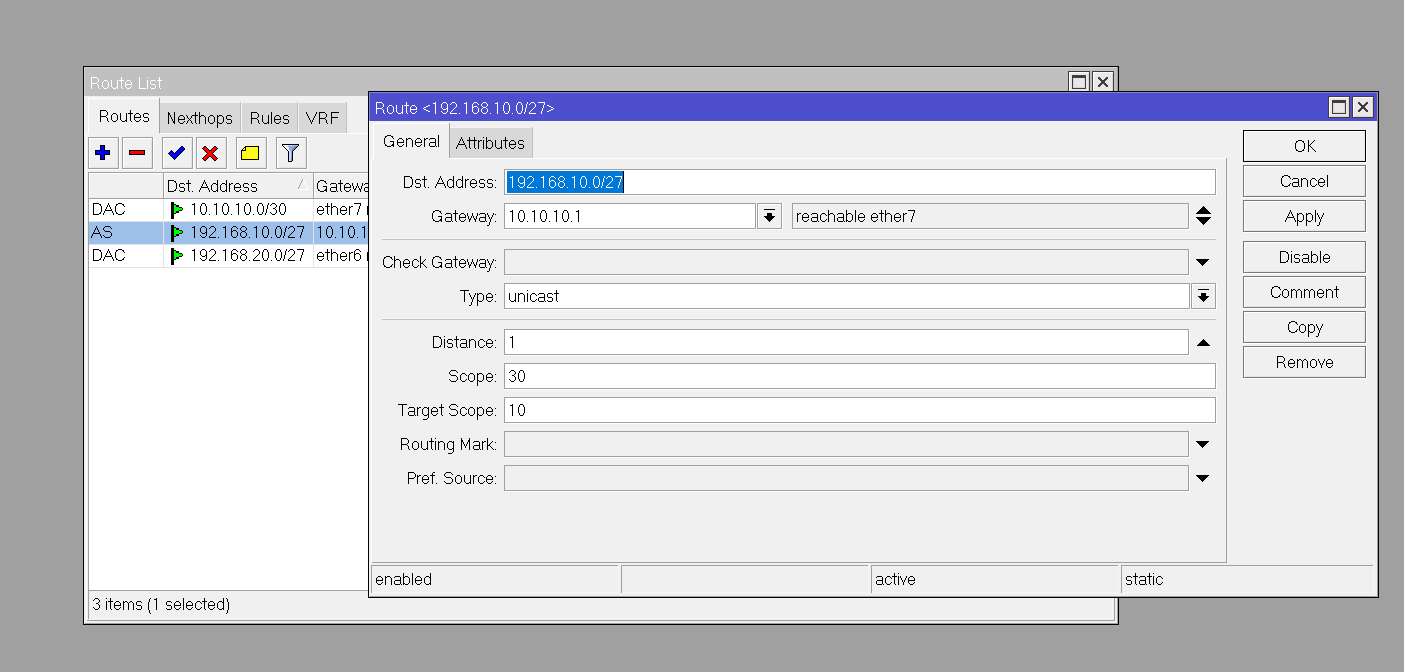
\includegraphics[width=0.5\linewidth]{P1/img/route list statis2.png}
            \caption{Route List 2}
            \label{fig:enter-label}
        \end{figure}
        
    \item Pada Network Setting laptop. Atur IP menjadi manual dan masukan IP Address yang diinginkan, netmask index /27 (255.255.255.224) dan gateway network yang sedang digunakan laptop. Lakukan untuk kedua laptop

    \item Pada laptop matikan Firewall agar package dari network tidak terblokir.

    \item Lakukan test Ping ke kedua Router dan laptop pada network yang berbeda. pada terminal kedua laptop.
        \begin{figure}[H]
            \centering
            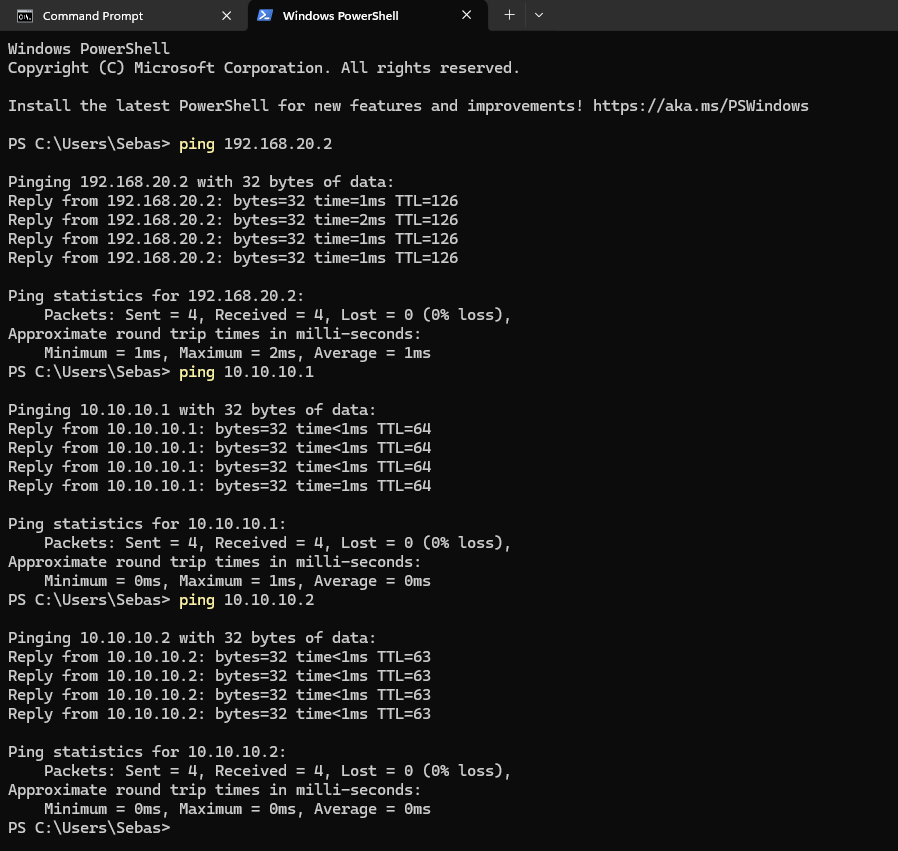
\includegraphics[width=0.5\linewidth]{P1/img/static.png}
            \caption{Static Ping Laptop 1}
            \label{fig:enter-label}
        \end{figure}
        \begin{figure}[H]
            \centering
            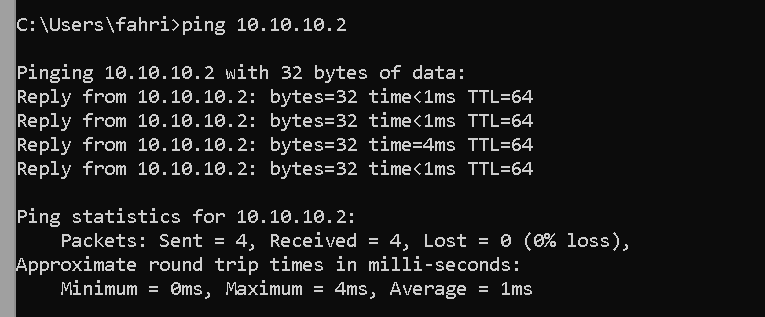
\includegraphics[width=0.5\linewidth]{P1/img/ping.png}
            \caption{Static Ping Laptop 2 ke Router 2}
            \label{fig:enter-label}
        \end{figure}
        \begin{figure}[H]
            \centering
            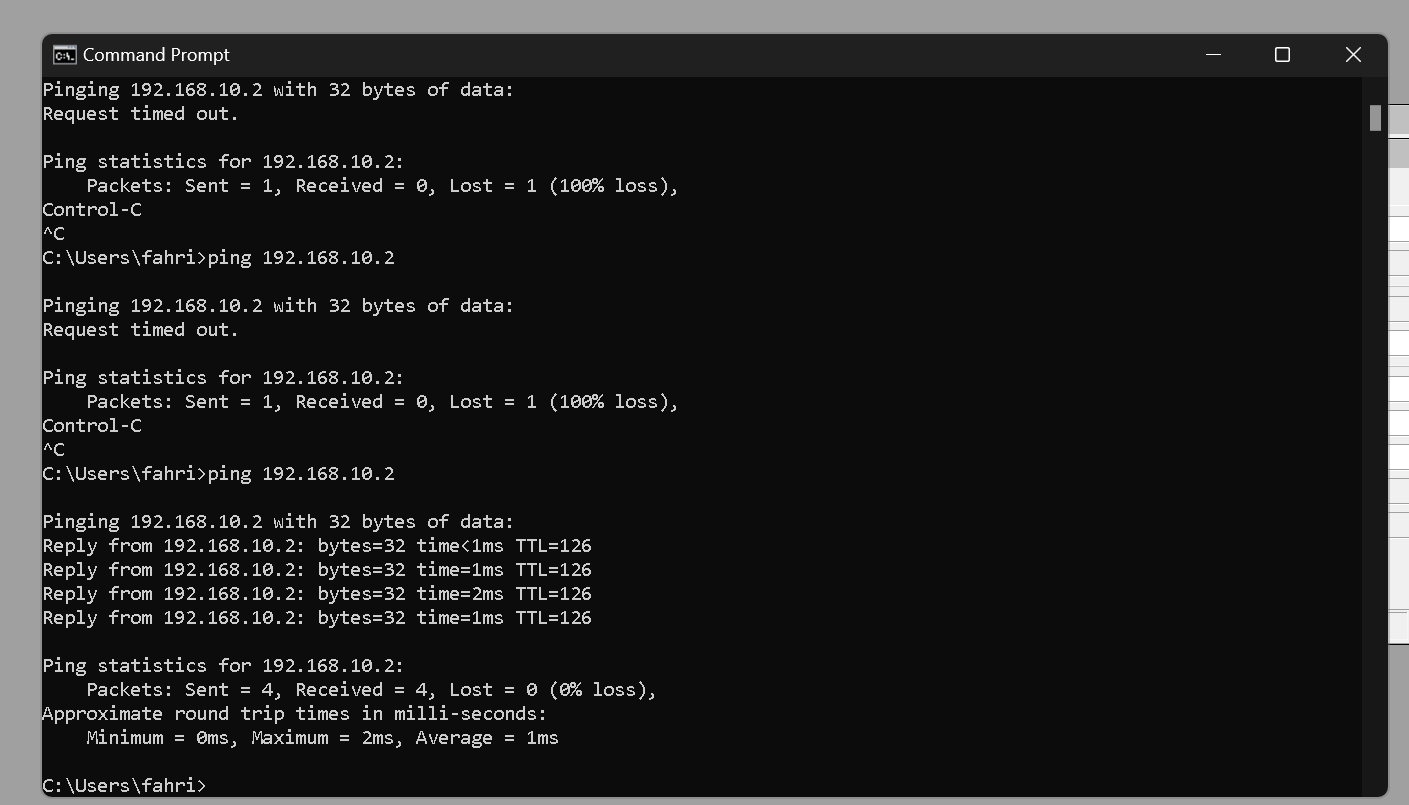
\includegraphics[width=0.5\linewidth]{P1/img/ping 2.png}
            \caption{Static Ping Laptop 2 ke Laptop 1}
            \label{fig:enter-label}
        \end{figure}
        \begin{figure}[H]
            \centering
            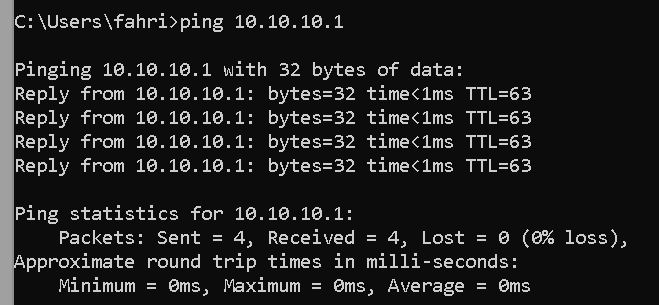
\includegraphics[width=0.5\linewidth]{P1/img/pingrouter2.png}
            \caption{Static Ping Laptop 2 ke Router 1}
            \label{fig:enter-label}
        \end{figure}
        
\end{enumerate}

\subsection{Dynamic Routing}
\begin{enumerate}

    \item Pada WinBox, Route List dari Static Routing Dihapus dengan menekan tombol (-).

    \item Buka menu IP dan pilih DHCP. Pada window DHCP server klik tombol DHCP Setup. Pilih interface ether6.

    \item Buka menu Routing dan pilih RIP. Tambahkan interface dan pilih Ether All. Set Receive V1-2, send ke V-2, Authentication none.
        \begin{figure}[H]
            \centering
            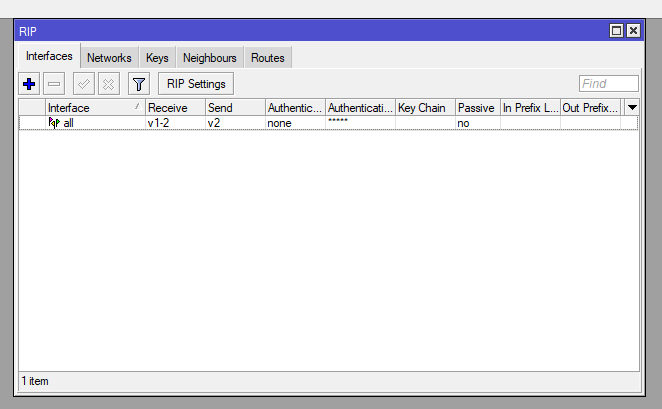
\includegraphics[width=0.5\linewidth]{P1/img/rip interfaces.png}
            \caption{RIP Interface Router 1}
            \label{fig:enter-label}
        \end{figure}
        \begin{figure}[H]
            \centering
            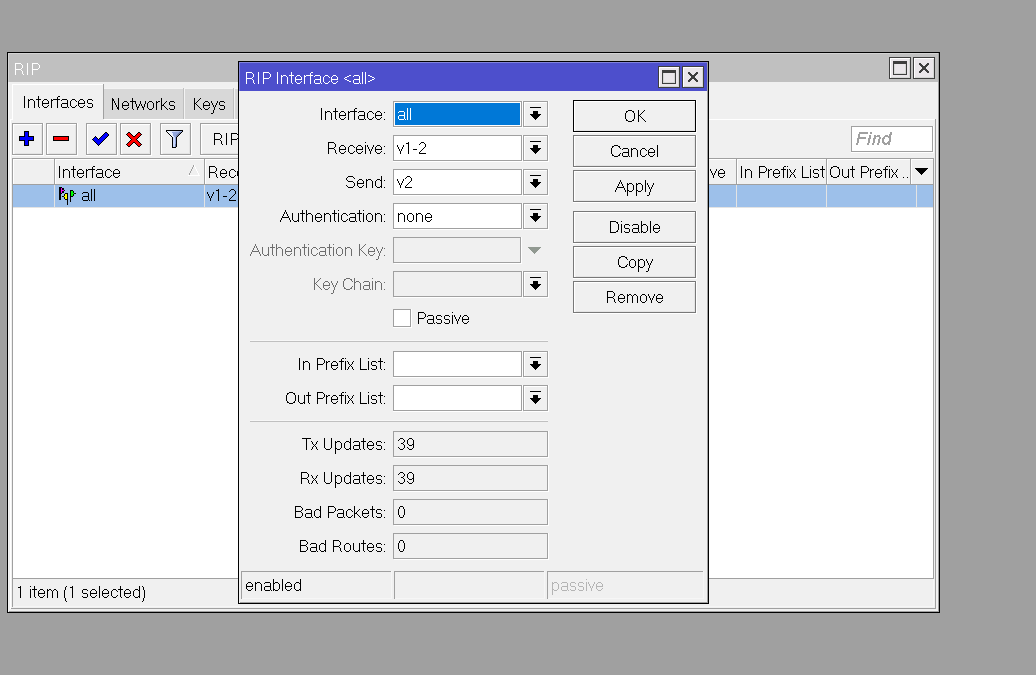
\includegraphics[width=0.5\linewidth]{P1/img/rip interfaces 2.png}
            \caption{RIP Inteface Router 2}
            \label{fig:enter-label}
        \end{figure}

    \item Pada menu RIP, pilih tab Networks dan masukan semua Network IP yang terhubung dengan router.
        \begin{figure}[H]
            \centering
            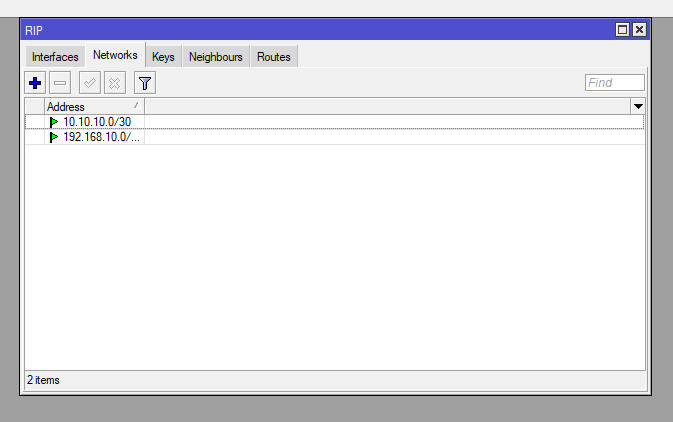
\includegraphics[width=0.5\linewidth]{P1/img/rip networks.png}
            \caption{RIP Network Router 1}
            \label{fig:enter-label}
        \end{figure}
        \begin{figure}[H]
            \centering
            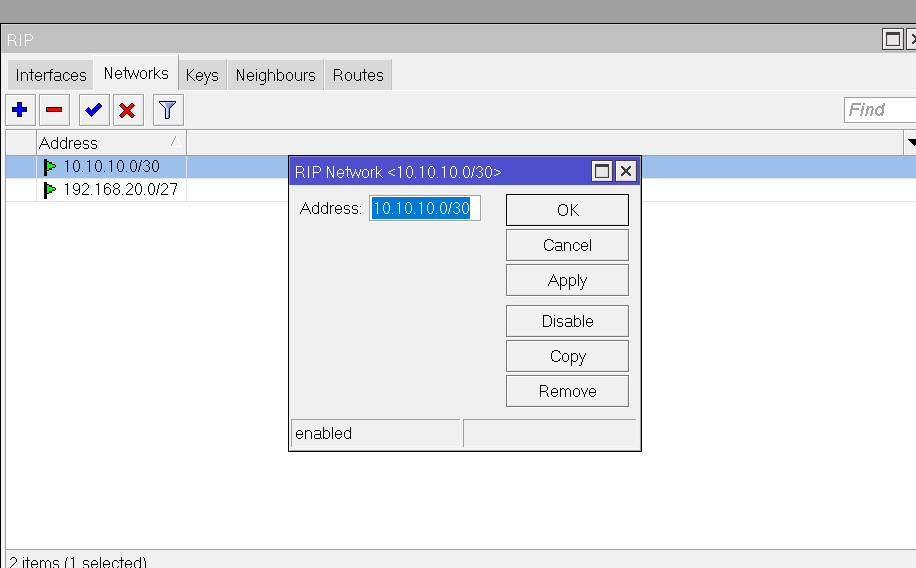
\includegraphics[width=0.5\linewidth]{P1/img/RIP Net.png}
            \caption{RIP Netwroks Router 2}
            \label{fig:enter-label}
        \end{figure}

    \item Pilih tab Negibours dan isi gateway dari laptop destinasi.
        \begin{figure}[H]
            \centering
            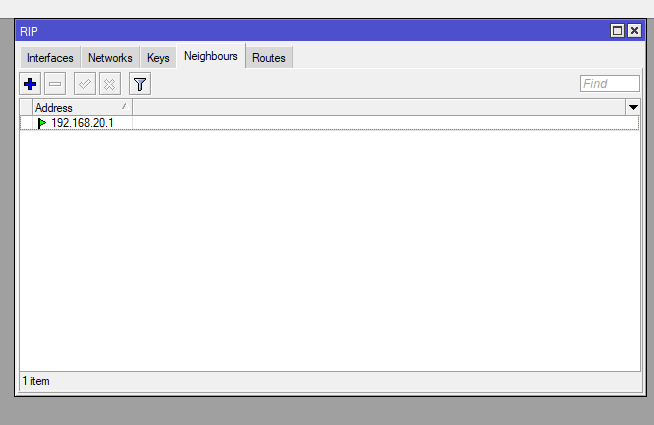
\includegraphics[width=0.5\linewidth]{P1/img/rip neighbours.png}
            \caption{RIP Neighbour Router 1}
            \label{fig:enter-label}
        \end{figure}
        \begin{figure}[H]
            \centering
            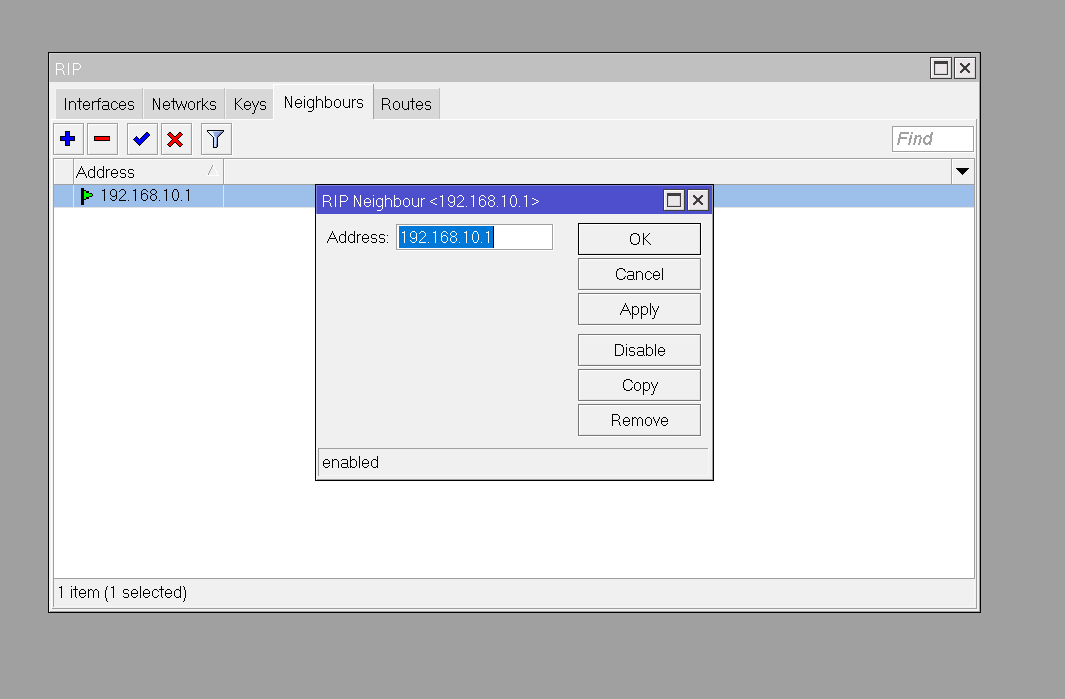
\includegraphics[width=0.5\linewidth]{P1/img/RIp Neighbvours.png}
            \caption{RIP Neigbour Router 2}
            \label{fig:enter-label}
        \end{figure}

    \item pada masing-masing laptop ubah IP Setting menjadi DHCP dan lakukan Test Ping ke antar Laptop, Router1, dan Router 2.
    \begin{figure}[H]
        \centering
        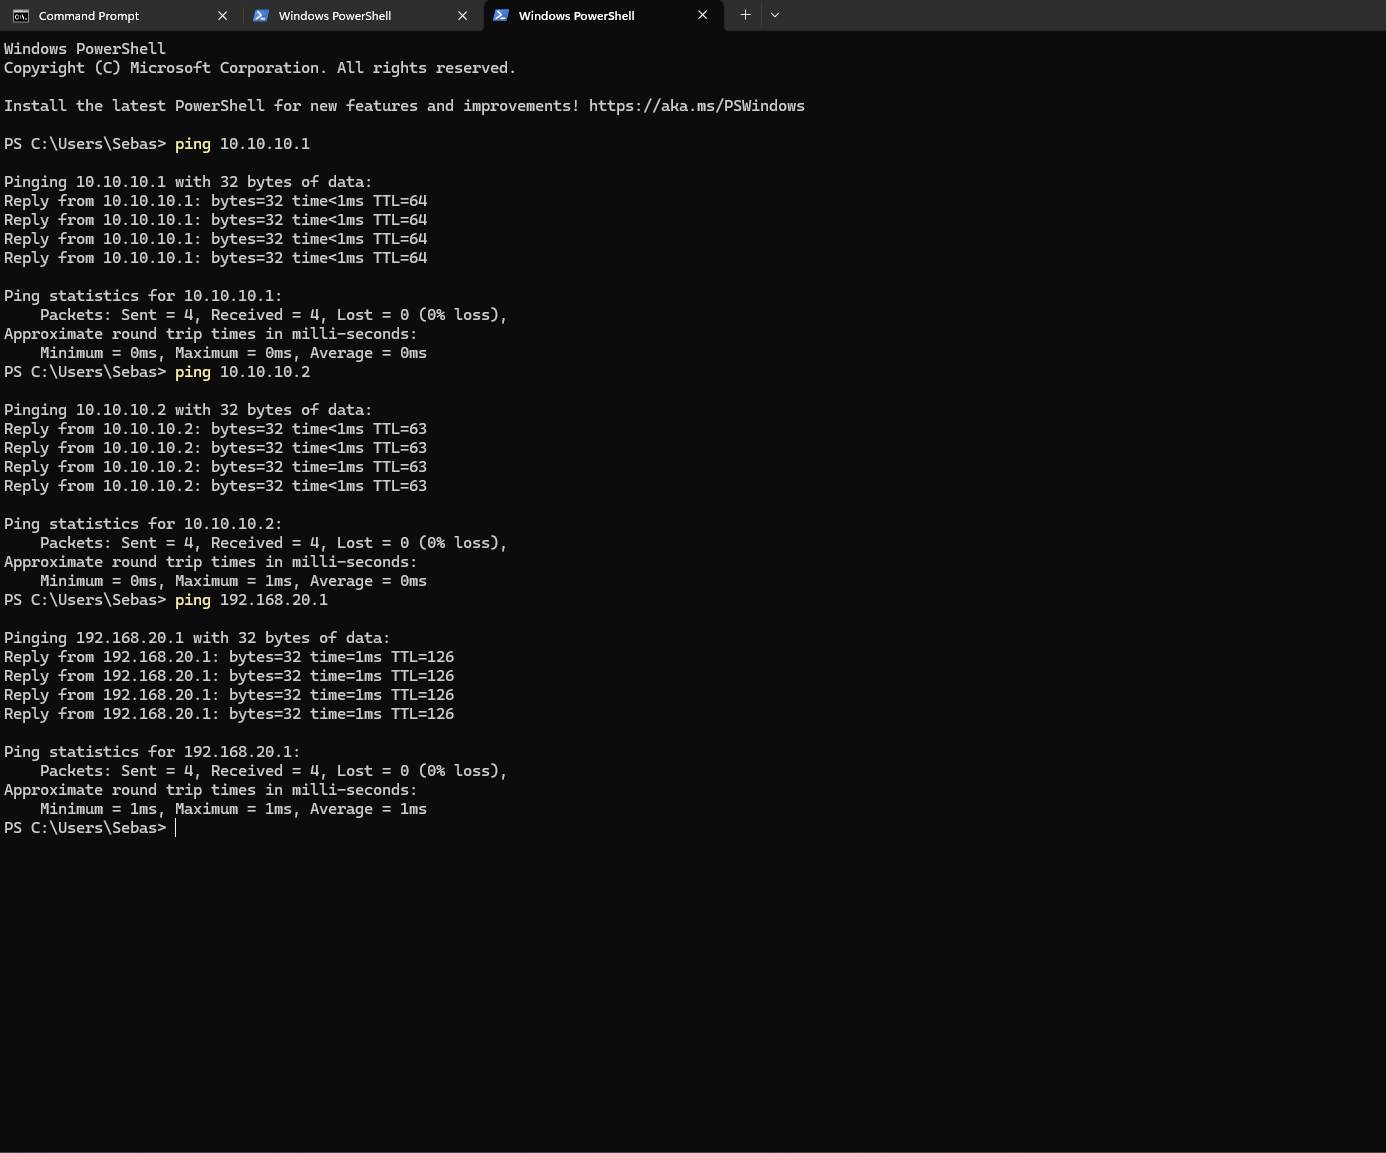
\includegraphics[width=0.5\linewidth]{P1/img/ping dynamic.png}
        \caption{Ping Dynamic Laptop 1}
        \label{fig:enter-label}
    \end{figure}
    
\end{enumerate}

\section{Analisis Hasil Percobaan}
Pada Percobaan 1 dilakukan crimping kabel UTP. Kabel UTP terdiri dari 8 kabel didalamnya. 8 kabel tersebut memiliki kegunaan masing-masing. Misal ada yang untuk transmit data TX(orange), receive data RX(Hijau), power (coklat). Terdapat 4 warna dimana ada kabel yang memiliki strip putih. Kabel yang memiliki strip putih menunjukan pasangan positif dari set warna tersebut. Terdapat beberapa Category untuk kabel UTP, Kabel UTP yang digunakan pada praktikum adalah Kabel UTP CAT5, dimana kabel tersebut tidak memiliki grounding pada kabel tersebut, sehingga pada LAN Tester LED yang mengetest kabel grounding tidak menyala.

Pada Percobaan 2 dilakukan configurasi routing static. Dilakukan dengan menggunakan 2 router dan 2 laptop. Topology yang digunakan pada praktikum ini menggunakan tiga network yaitu Network 10.10.10.0 untuk IP network antar router dan Network 192.168.10.0 untuk IP Network antar Router 1 dengan Laptop 1, Netwrok 192.168.20.0 untuk IP Network antar router 2 dengan Laptop 2. Pada Network antar router menggunakan CIDR /30 yang melimit penggunaan menjadi 2 usable IP dan pada Network rounter dengan perangkat user menggunakan CIDR /27 yang melimit user menjadi 30 usable IP. Untuk mengatur dan mengassign IP Address dengan Networknya yang digunakan dapat dilakukan pada router dan menambahkannya pada address list beserta dengan interface yang terhubung pada router tersebut, misal ether7 terhubung antar router maka pada address list kita assign dengan Network IP 10.10.10.0 dengan Address dari gateway misal 10.10.10.1/30. Hal tersebut dapat dilakukan juga untuk ke network perangkat user. Untuk menentukan IP tersebut perlu dituju kemana maka dapat diatur pada Route List. Route List menunjukan list dari Address yang dapat diakses melalui interface. Route dapat ditambahkan dengan memasukan destination address dan gateway yang ingin dituju. Pada saat melakukan praktikum, ketika melakukan ping antar laptop, packets dari laptop pengirim tidak dapat diterima oleh laptop penerima, hal ini dikarenakan Firewall yang memblokir packets yang masuk.

Pada Percobaan 3 dilakukan configurasi routing dynamic. Routing Dynamic memungkinkan perangkat untuk mengassign IP Address-nya secara otomatis dan membentuk topologi network secara otomatis. Karena dapat dilakukan secara otomatis maka diperlukan Protocol tertentu untuk memiliki standar untuk berbagi informasi, maka digunakan Routing Information Protocol (RIP). Pada menu RIP dapat disetting interface yang akan digunakan protocol tersebut serta dapat memilih Network serta Gateway yang menggunakan protocol ini.

\section{Hasil Tugas Modul}
\begin{enumerate}
    \item Cisco Packet Tracer
    \begin{figure} [H]
        \centering
        \includegraphics[width=1\linewidth]{P1//img/{F2D18938-F436-432D-9696-932025FDBE6D}.png}
        \label{Ping}
    \end{figure}
    \begin{figure}[H]
        \centering
        \includegraphics[width=0.5\linewidth]{P1/img/{DECA2917-4647-44B6-B80F-7EB2026B0806}.png}
        \label{fig:enter-label}
    \end{figure}
    \item Banyak istilah yang tidak umum dan belum dipahami. Serta kegunaan dan tujuan dari setiap step pada praktikum.
\end{enumerate}

\section{Kesimpulan}
Pada Static Routing, diperlukan untuk mengassign IP dan Routing secara manual. Sehingga kita perlu menambahkan address dari masing-masing network dan mengatur index-nya. Dari address tersebut dihubungkan melalui routing melalui interface yang tersambung.
Pada Dynamic Routing, semua routing dan IP sudah diatur secara otomatis. Kita hanya perlu mensetting protocol yang digunakan.

\section{Lampiran}
\subsection{Dokumentasi saat praktikum}
\begin{figure}[H]
    \centering
    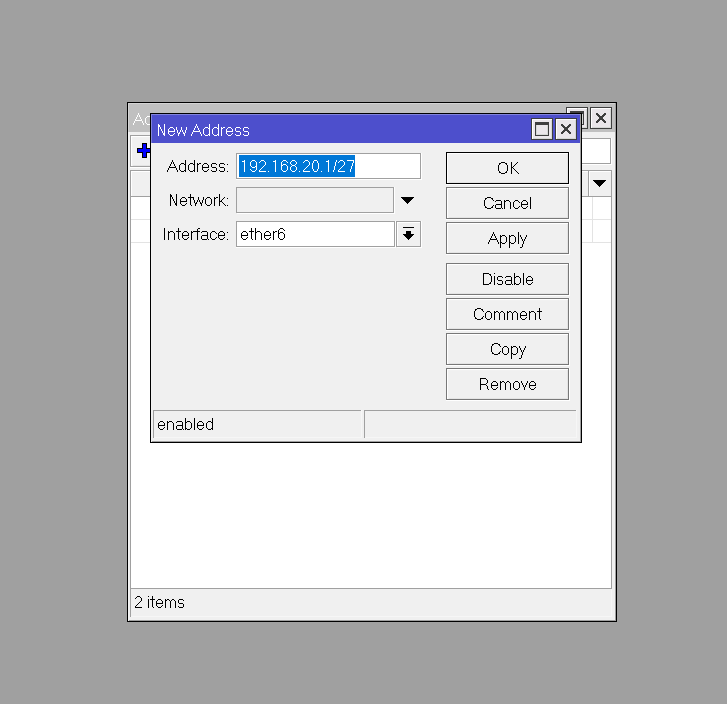
\includegraphics[width=0.5\linewidth]{P1/img/Address Laptop Router 2.png}
    \label{fig:enter-label}
\end{figure}
\begin{figure}[H]
    \centering
    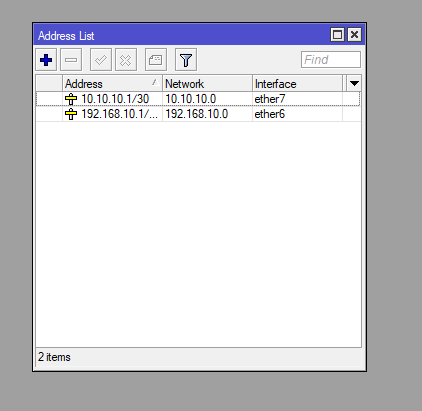
\includegraphics[width=0.5\linewidth]{P1/img/address list static.png}
    \label{fig:enter-label}
\end{figure}
\begin{figure}[H]
    \centering
    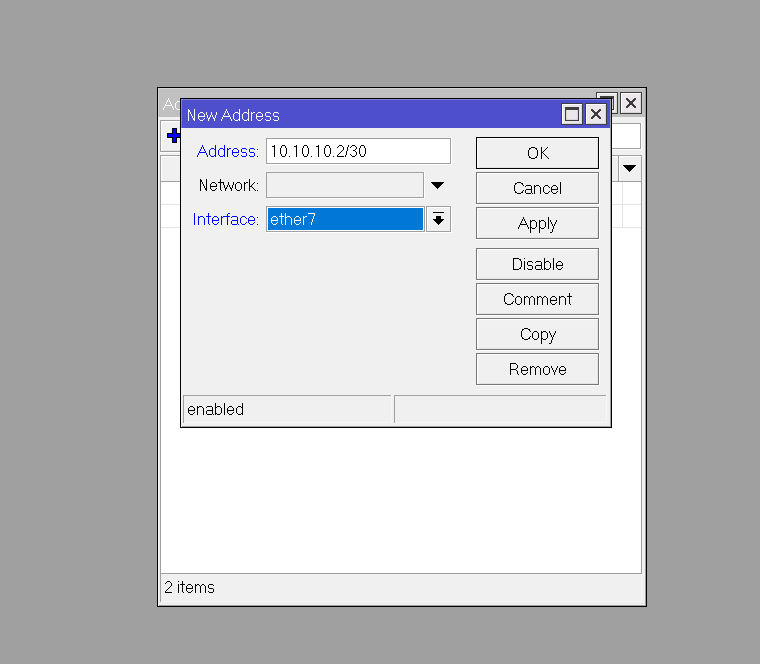
\includegraphics[width=0.5\linewidth]{P1/img/Address Router Router 2.png}
    
    \label{fig:enter-label}
\end{figure}
\begin{figure}[H]
    \centering
    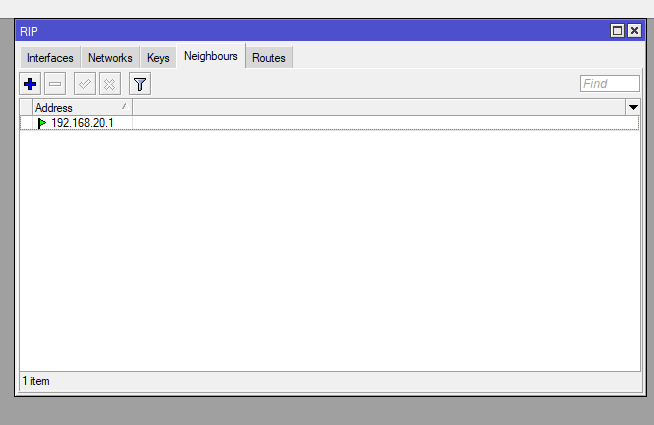
\includegraphics[width=0.5\linewidth]{P1/img/rip neighbours.png}
    
    \label{fig:enter-label}
\end{figure}
\begin{figure}[H]
    \centering
    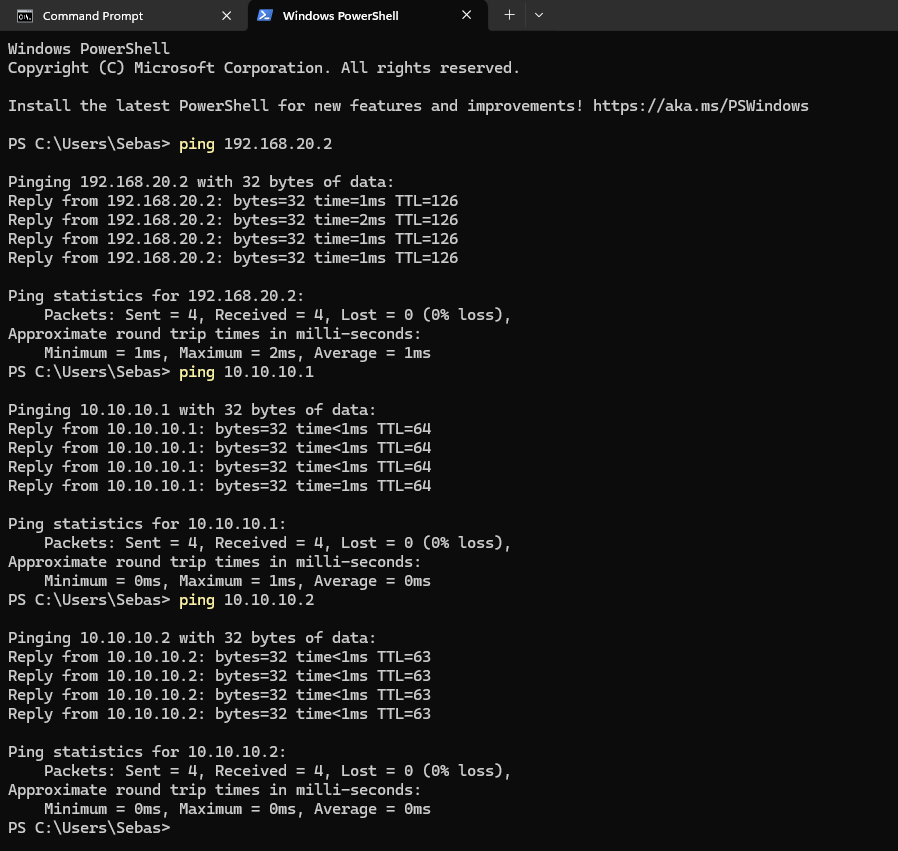
\includegraphics[width=0.5\linewidth]{P1/img/static.png}
    
    \label{fig:enter-label}
\end{figure}
\begin{figure}[H]
    \centering
    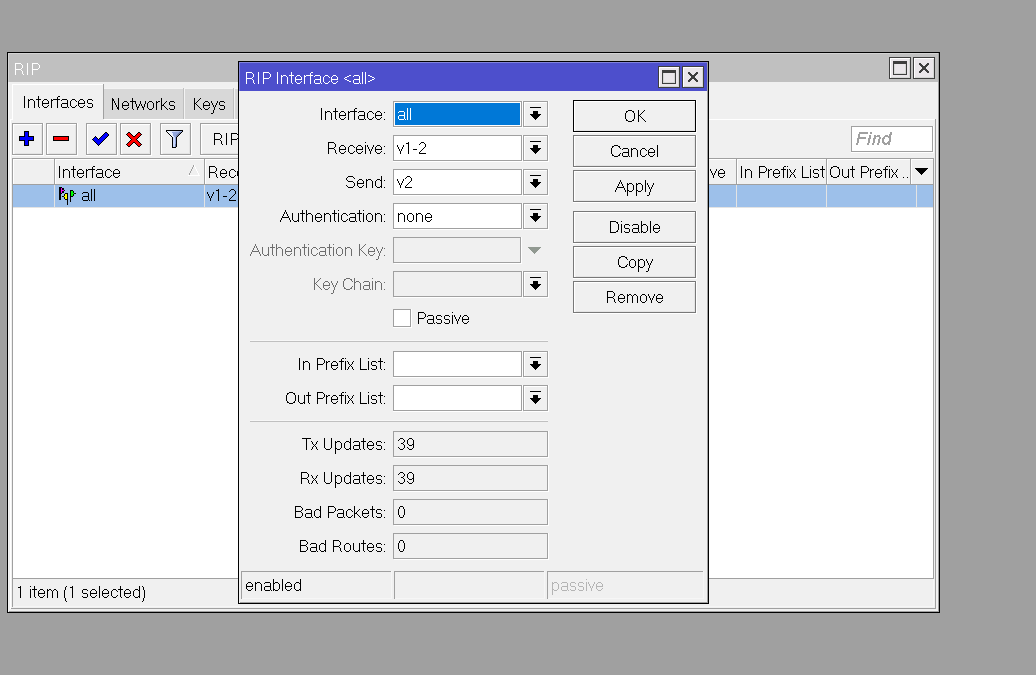
\includegraphics[width=0.5\linewidth]{P1/img/rip interfaces 2.png}
    \label{fig:enter-label}
\end{figure}
\begin{figure}[H]
    \centering
    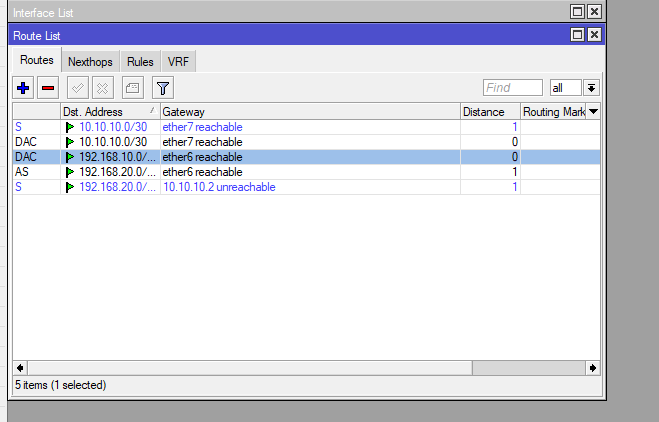
\includegraphics[width=0.5\linewidth]{P1/img/route list statis.png}
    \label{fig:enter-label}
\end{figure}
\subsection{Hasil Challenge Modul}
Challenge yang dilakukan, membuat Routing Dynamic antar router dan laptop dengan perantara Switch pada network Router - Laptop. Diberikan 4 router, salah dari 2 router harus dijadikan Switch. Caranya dengan mengubah mode router menjadi bridge. Serta diminta untuk usable IP yang dibutuhkan ditambah. Caranya dengan mengubah CIDR IP Network pada main router, kemarin menjadi /24 sehingga usable IP menjadi 254 client.
\begin{figure}[H]
    \centering
    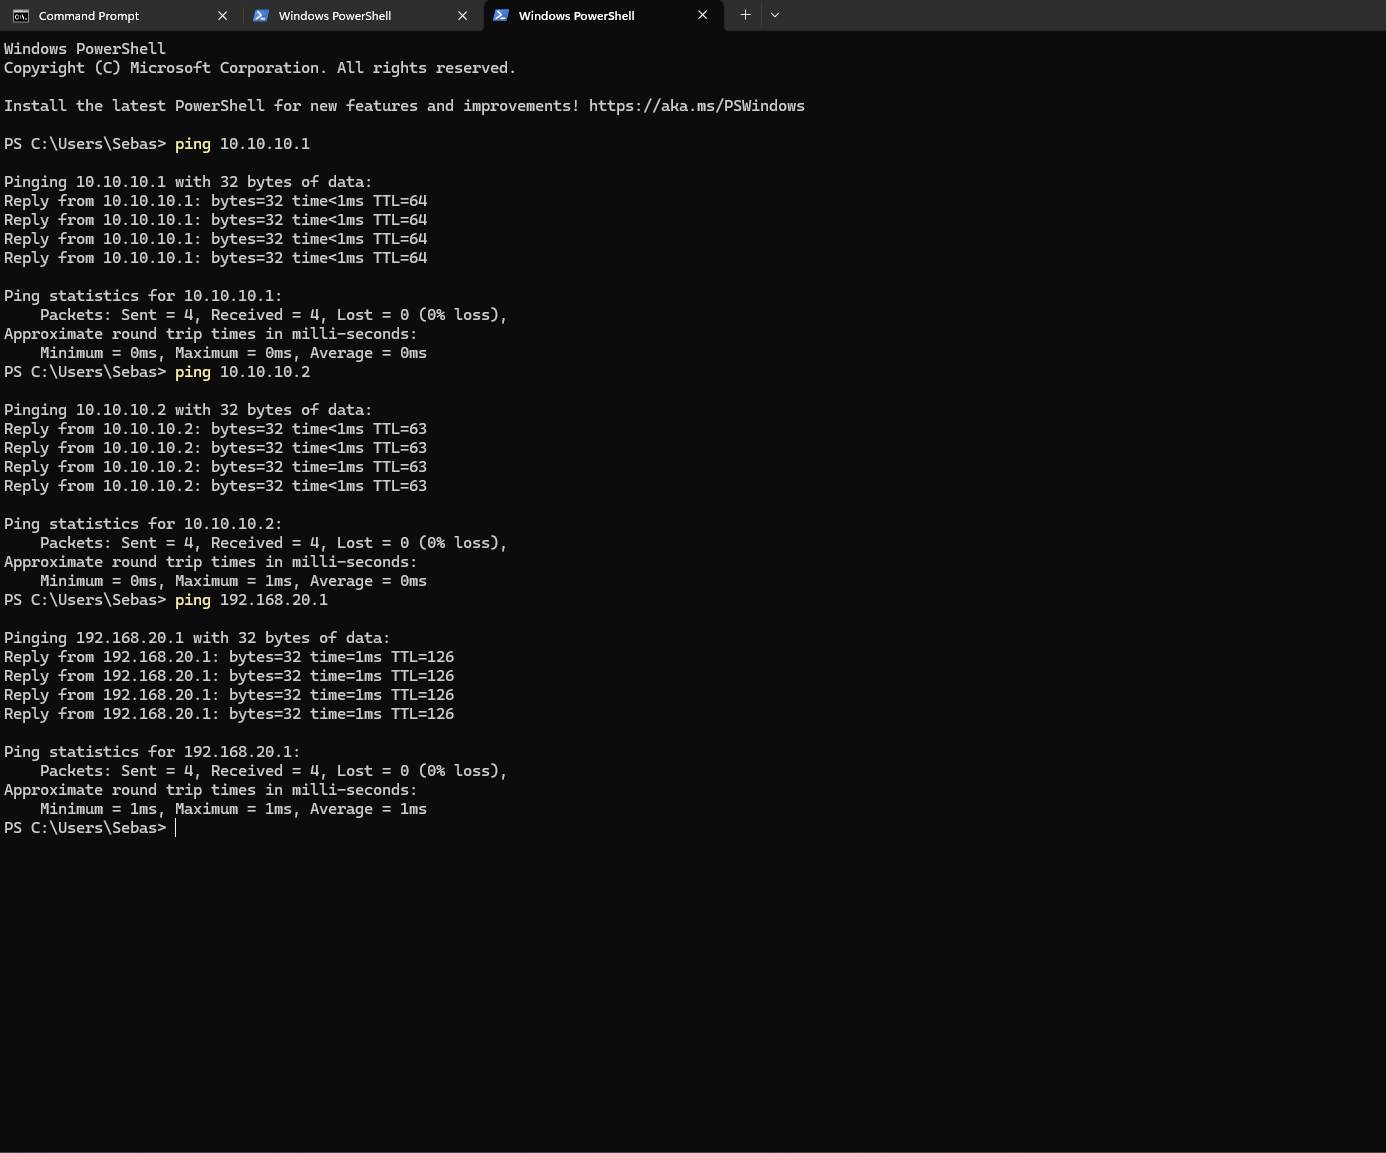
\includegraphics[width=0.75\linewidth]{P1/img/Screenshot 2025-05-10 164954.png}
    \caption{Challenge}
    \label{fig:enter-label}
\end{figure}